\paragraph{How to determine molecules' distance}
To determine the distance between molecules, one has to carefully choose the points of interest. As a problem of STM imaging the contour of the molecules sometimes appears as more or less fuzzy shape. There is no sharp edge that one could take as start or end point of the profile. Therefore the center of the molecule is often used as reference point to measure the distance between two molecules (compare fig. \ref{fig:distance-molecules}). As the molecule has a square footprint, one can use the center in one direction (along profile 2/3) to determine the center in the other direction (profile 1). As one can see the three profiles match leading to a consistent center of the dimer. This is also shown as depression in profile 1. 

\begin{figure}[]
	\centering
	\subfigure[Molecule with chosen profiles (1-3) indicated as white lines.]{
		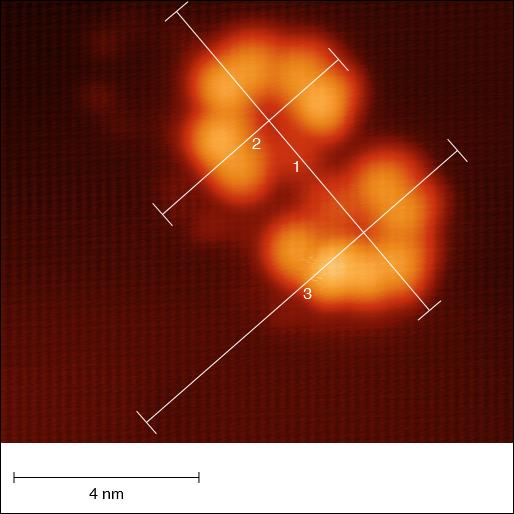
\includegraphics[width=0.45\textwidth]{./images/F150612-163956-dimer-loose.jpg}
	} \quad
	\subfigure[Profiles 1-3 indicated in a).  Local minima in profile 2/3 indicate central positions in profile 1.]{
		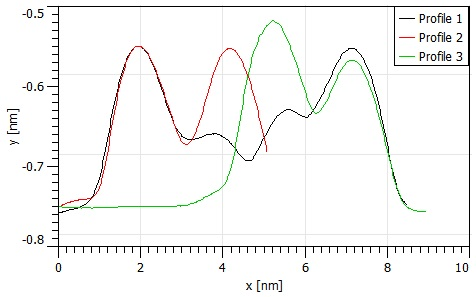
\includegraphics[width=0.45\textwidth]{./images/F150612-163956-profile-dimer-loose.jpg}
	}
	\caption{Sketch of how to determine the distance between two molecules. As the molecule is square (with the exception of one direction, one can determine the center of the molecule by comparing two \SI{90}{\deg} rotated profiles. Profile 1 goes through the symmetry axis, while profile 2 and 3 intersect profile 1 at the center. As the profile 2 and 3 look the same when starting at the buthyl groups, one can use the depression in profile 2 and 3 to determine the center of the molecule in profile 1.}
	\label{fig:distance-molecules}
\end{figure}